% !TEX root = Bachelorarbeit_Paul_Zilewitsch.tex
\section{Microsoft Exchange Server}

\subsection{Grundlagen}
\noindent 
Der  Microsoft Exchange Server ist eine serverseitige Anwendung, die den Nachrichtenaustausch und die Zusammenarbeit im Unternehmen erleichtern soll.\footnote{Vgl. \citeauthor{Joos} (\citeyear{Joos}), S. 26.} Im Juni 1996 wurde die erste Version von Microsoft Exchange veröffentlicht. Sie löste das Mailsystem MS Mail ab, da dieses für einen Gebrauch mit über 500 Postfächern nicht ausgelegt und somit für größere Unternehmen nicht mehr sinnvoll war. Dieser Wechsel der Software wurde passend durch den Namen Exchange beschrieben, da es so viel heißt wie \enquote{Austausch}. Ziel des Microsoft Exchange Servers ist es, Nachrichten zu verarbeiten und zu verwalten. Obwohl Exchange ein Mailserver ist, können neben E-Mails auch Termine angelegt oder Aufgaben vergeben werden. Somit wäre es denkbar, Exchange als zentrale Anlaufstelle der Unternehmenskommunikation einzusetzen.\newline
Microsoft Exchange ist klar in den Bereich Groupware einzuordnen. Gropuware-Software wird vor allem zur Unterstützung der internen als auch der externen Unternehmenskommunikation genutzt. Ellis, Gibbs und Rein beschreiben die bekannteste Form von Groupware als ein 
\enquote{computer-based message system, which supports the asynchronous exchange of textual messages between groups of users.}\footnote{\citeauthor{Ellis} (\citeyear{Ellis}), S. 38 ff.} Also ein Computersystem für den asynchronen Austausch von von Textnachrichten innerhalb einer Gruppe. Meistens sind dies Arbeitsgruppen im Unternehmensumfeld. Mircosoft Exchange erfüllt dieses Kriterium. Vorausgesetzt die Benutzer verfügen über eine Client-Software.\newline
Um auf die Inhalte des Microsoft Exchange Servers zugreifen zu können, benötigt jeder Benutzer eine Client-Software. Verwaltung des Postfaches, Zugriff auf öffentliche Ordner und natürlich auch Empfangen und Senden von E-Mails sind die Hauptziele einer Client-Software. Im Anhang auf Seite~\pageref{Exchange_Verbindungen} findet man eine Abbildung, die eine umfassende Übersicht verschiedener Clients darstellt. Diese Übersicht ist nicht Vollständigkeit, bildet aber dennoch die am häufigsten verwendeten Client-Systeme ab.\newline
Am bekanntesten ist sicher der Microsoft Outlook-Client. Aus diesem Grund wird die Verbindung eines Clients mit dem Exchange Server am Beispiel des Outlook-Clients erläutert. Outlook kommuniziert nach dem RPC-Prinzip mit dem Exchange Server. Die Variante RPC über TCP/IP  gilt zwar seit Exchange 2013 als veraltet, ist aber für das nähere Verständnis durchaus wichtig, da alle Weiterentwicklungen RPC im Hintergrund weiter nutzen. RPC bedeutet "Remote Procedure Call" und wird verwendet, um eine Verbindung zu einem Dienst eines Servers herzustellen. Als Übertragungsprotokoll fungiert TCP/IP (Transfer Control Protocol/Internet Protocol).\footnote{Website: \cite{MSXrpc}}Um die Kommunikation von RPC über TCP/IP zu verstehen, ist die nachfolgende Abbildung hilfreich.

\begin{figure}[h!]
\centering
	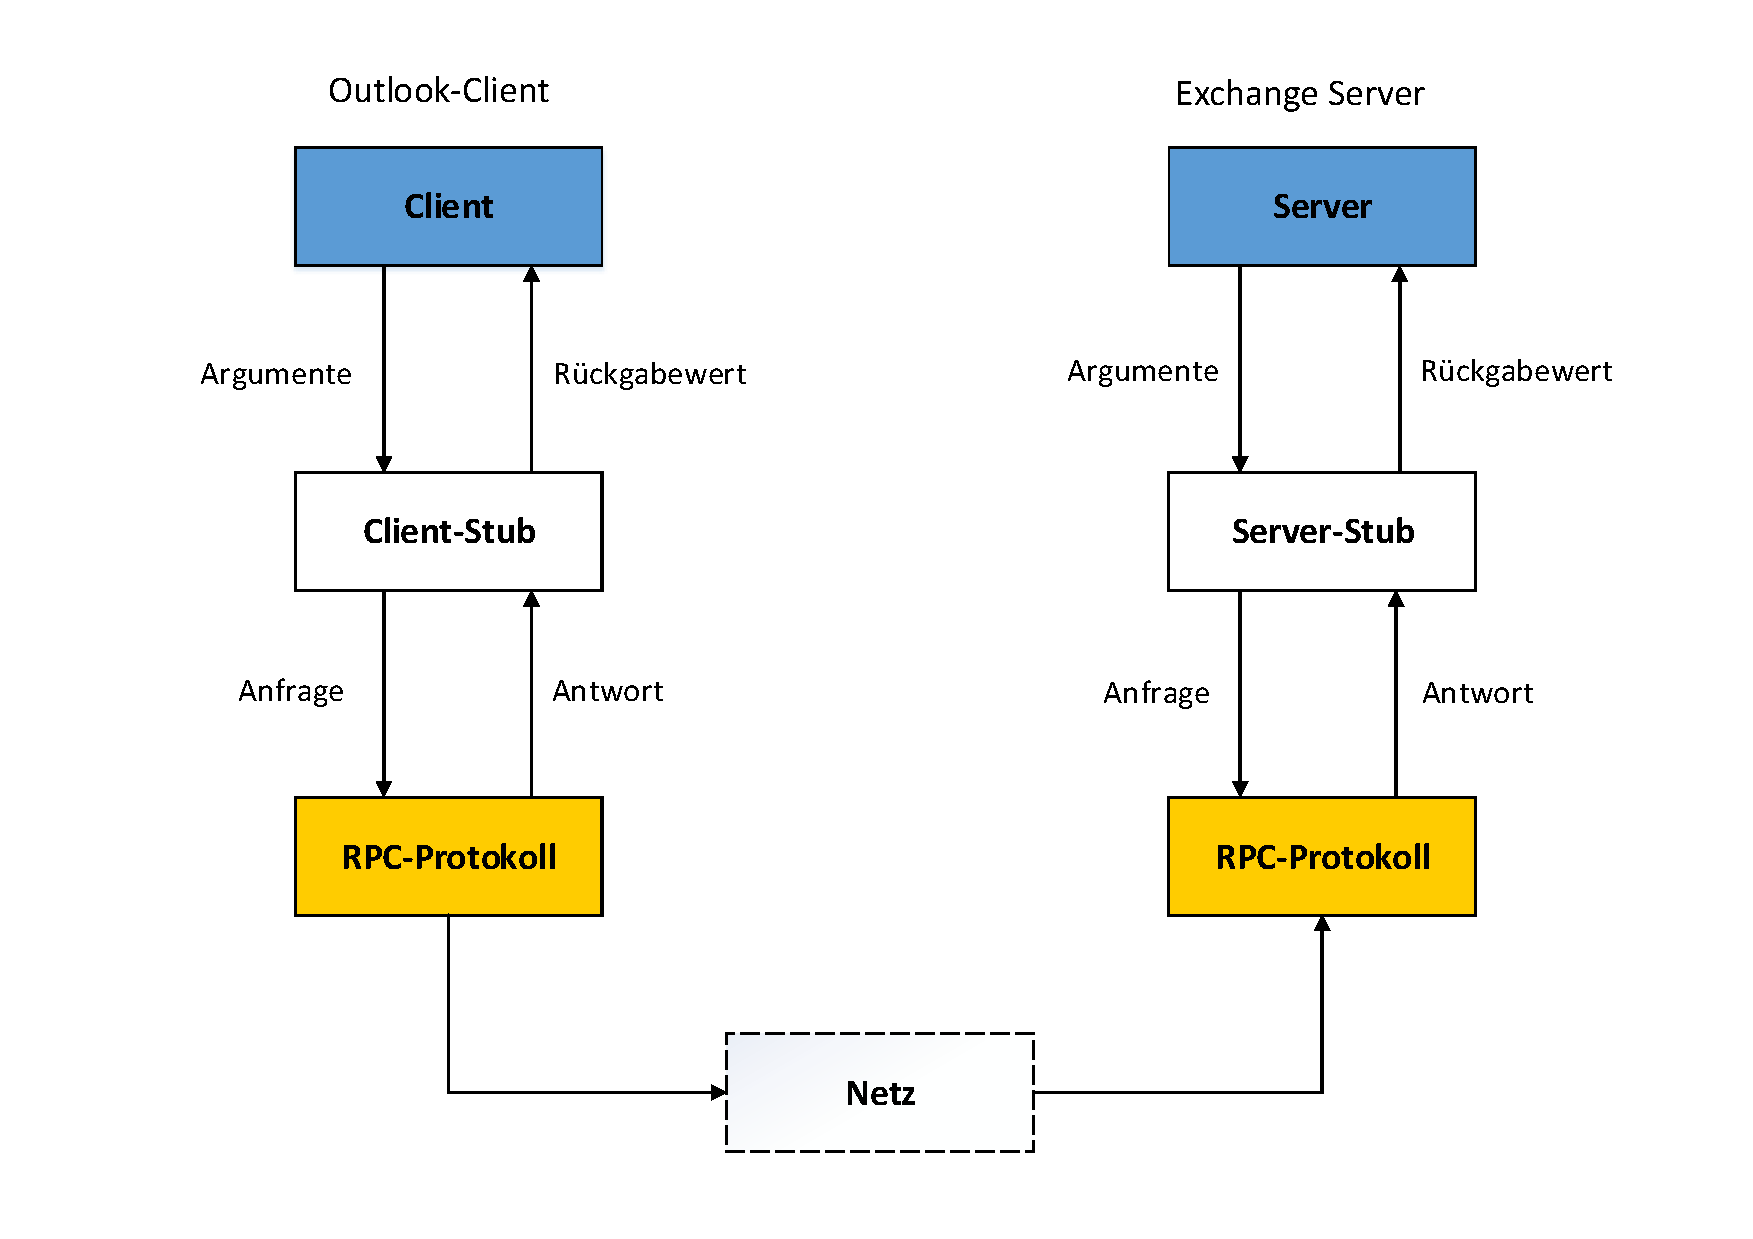
\includegraphics[width=0.55\textwidth]{Abbildungen/RPC_TCP.pdf}
	\caption[Aufbau einer klassischen RPC Verbindung]{Aufabu einer klassischen RPC Verbindung,    in Anlehnung an:\\https://technet.microsoft.com/de-de/library/e8feb37e-f3a9-4f26-bed0-6583d8a110ed}
	\label{fig:RPC_TCP}
\end{figure}

\noindent 
Der Client ruft eine Prozedur mit spezifischen Argumenten (Eingabeparameter) auf. Der Client-Stub aktiviert eine gleichnamige Prozedur und wandelt die Argumente in ein plattformunabhängiges Datenformat um. Die Daten werden dann über das Netz mithilfe des TCP/IP-Protokolls an den Server geschickt. Dort erhält der Server-Stub die Anfrage und wandelt die Argumente in das lokale Format des Servers um. Nun ruft der Server die gewünschte Prozedur mit den Eingabeparametern auf und der Rückgabewert kehrt in den Server-Stub zurück. Nach einer erneuten plattformunabhängigen Umwandlung der Datenformate, wird die Antwort an den Client-Stub geschickt. Im letzten Schritt erhält der Client die in das lokale Format umgewandelte Antwort (Rückgabewerte) auf seine Anfrage.\footnote{Vgl. \citeauthor{Schneider} (\citeyear{Schneider}), S.406 f.}\newline
Ab Exchange 20013 wird der Datenaustausch zwischen dem Outlook-Client und dem Exchanger Server standardmäßig über RPC/HTTP (auch Oulook Anywhere genannt) geregelt. Wie der Name schon vermuten lässt, läuft die gesamte Kommunikation bei dieser Variante über HTTP bzw. HTTPS. Somit kann über das Internet auf den Exchange Server zugegriffen werden. Outlook Anywhere ist besonders für Mitarbeiter geeignet, die von zu Hause auf ihr Exchange-Postfach zugreifen möchten, da sie sich nicht im Unternehmensnetzwerk befinden müssen.\footnote{Vgl. \citeauthor{Joos} (\citeyear{Joos}), S. 33, S. 254.}

\begin{figure}[h!]
\centering
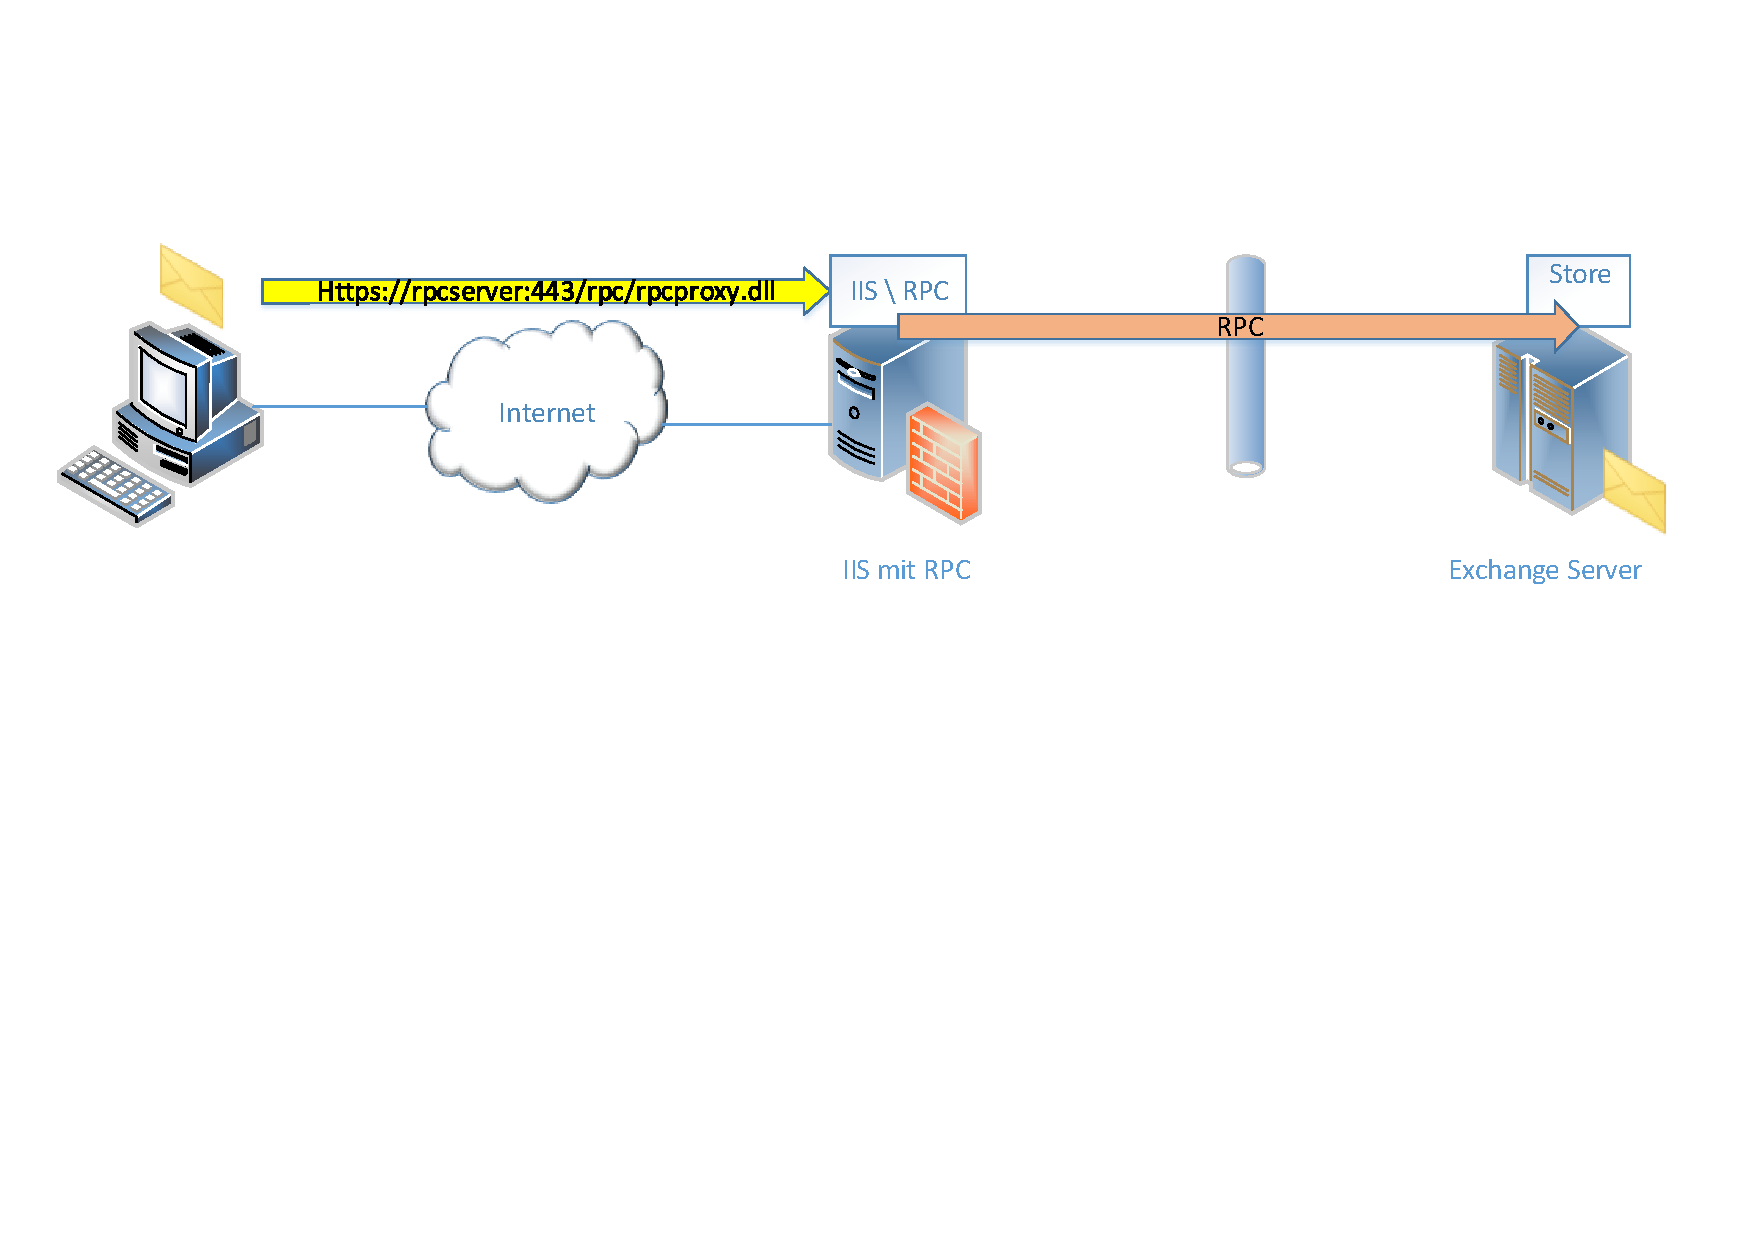
\includegraphics[width=0.65\textwidth]{Abbildungen/RPC_HTTP.png}
	\caption[RPC over HTTP Prinzip]{RPC over HTTP Prinzip,  in Anlehnung an:http://
	www.msxfaq.de/clients/oagrundlagen.htm}
	\label{fig:RPC_HTTP}
\end{figure}

\noindent
In der Abbildung \ref{fig:RPC_HTTP} sieht man deutlich, dass der Outlook-Client über HTTPS mit dem IIS kommuniziert, auf dem ein virtuelles RPC-Verzeichnis existiert. Der IIS ist eine Microsoft-Webserverplattform, die Webanwendungen und Dienste bereitstellen und verwalten kann.\footnote{Vgl. \citeauthor{Volodarsky} \citeyear{Volodarsky}, S.3.} Der IIS wiederum, baut über einen RPC-Proxy eine Verbindung mit dem Exchange Server auf. Wichtig ist hierbei, dass die Kommunikation des Clients sich auf HTTP oder HTTPS beschränkt.\footnote{Website:  \citeauthor{MSXoutlook} (abgerufen am: 13.06.2016)}


\subsection{Exchange Web Services}
\noindent
Die Grundlagen von Mircosoft Exchange Server sind geklärt. Doch wie können nun Programmierer über Quellcode auf den Exchange Server zugreifen. Hierfür hat Mircosoft im Laufe der Jahre eine Reihe von Programmierschnittstellen bereitgestellt. Eine Schnittstellen zur Anwendungsprogrammierung wird als API (englisch application programming interface) bezeichnet. Es ist nicht nötig, alle Programmierschnittstellen zu erläutern, da eine Vielzahl der APIs keine Verwendung mehr finden oder nicht mehr unterstützt werden. Zu Informationszwecken befindet sich jedoch im Anhang auf Seite~\pageref{API_Geschichte} eine Übersicht einiger Programmierschnittstellen ab dem Jahr 1992. Ab Exchange 2007 setzt Microsoft immer mehr auf den Exchange Web Services (kurz EWS) als Programmierschnittstelle und baut diese seitdem weiter aus.\footnote{Website: \citeauthor{MSXews} (abgerufen am: 14.06.2016)}
Redmond schreibt im Handbuch Exchange 2010: 
\enquote{Abgesehen von Windows PowerShell liegt der Schwerpunkt für die meisten Entwickler jetzt auf der API EWS (Exchange-Webdienste), die in Exchange Server 2007 eingeführt wurde.}\footnote{\citeauthor{Redmond} \citeyear{Redmond}, S.634.}
Er macht deutlich, dass EWS die erste Anlaufstelle für Entwickler ist. Eine weitere Programmierschnittstelle namens REST API erschien 2015 mit Office 365. Der REST API wird aber keine weitere Beachtung geschenkt, da sie lediglich in der Office 365-Umgebung Anwendung findet.\footnote{Website: \citeauthor{MicrosoftAPI} (abgerufen am: 15.06.2016)}


\subsubsection{Funktionsweise}
\noindent
Standardmäßig bildet das Simple Object Access Protocol (kurz SOAP) eine Grundlage für Web-Services. Schneider beschreibt SOAP als \enquote{ein RPC-Mechanismus, bei dem die übertragenen Daten im XML-Format codiert werden.}\footnote{\citeauthor{Schneider} \citeyear{Schneider}, S.407.}
Schill und Springer schreiben genauer: \enquote{Das objektorientierte Kommunikationsprotokoll SOAP ermöglicht die Kommunikation zwischen heterogenen Diensten unter interner Nutzung
des Hypertext Transfer Protocol (HTTP) und mit Kodierung der Parameter in der eXtensible Markup Language (XML).}\footnote{\citeauthor{Schill} \citeyear{Schill}, S.69.}
Auch die Exchange Web Services funktionieren nach diesem Prinzip.\footnote{Website: \citeauthor{MicrosoftSDK} (abgerufen am: 13.06.2016)}
 
\noindent
Mit Exchange 2007 wurde erstmals der Exchange Web Services  bereitgestellt und löste nach und nach andere APIs ab. Die nachfolgende Abbildung zeigt, wie sich EWS seit 2007 entwickelt hat.

\begin{figure}[h!]
\centering
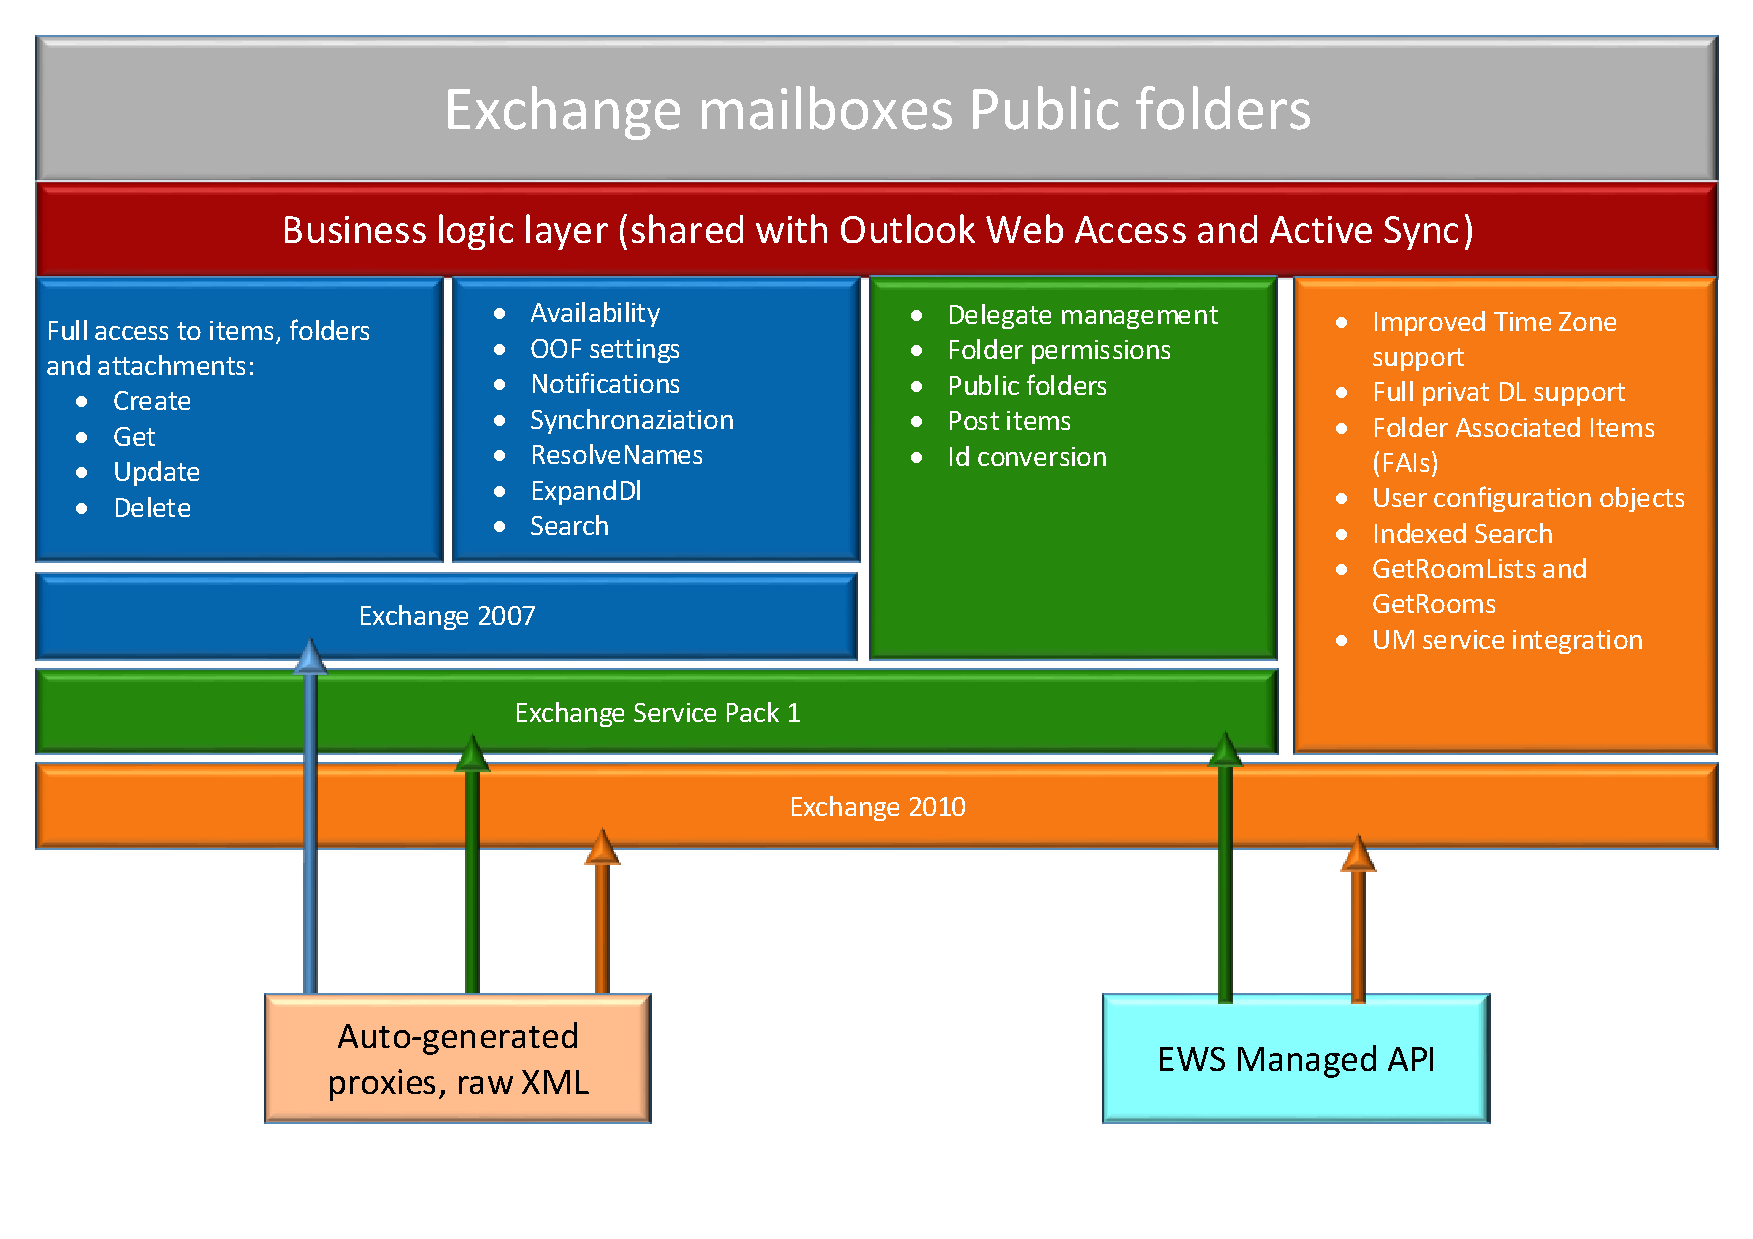
\includegraphics[width=0.65\textwidth]{Abbildungen/EWS_Funktionsumfang.pdf}
	\caption[EWS Funktionsumfang]{EWS Funktionsumfang, Quelle: http://www.msxfaq.de/code/
	ews.htm}
	\label{fig:EWS_Funktionsumfang}
\end{figure}

\noindent
EWS bietet einen großen Funktionsumfang und ist somit eine hervorragende Möglichkeit auf die Daten des Exchange Servers zuzugreifen. Aus diesem Grund haben sich die Entwickler der KMS Computer GmbH für diese Programmierschnittstelle entschieden.

\subsubsection{Derzeitige Verwendung in GEBman 10}
\noindent
Um bei der Implementierung den Exchange Web Service nutzen zu können, musste die Microsoft Exchange Web Services Managed API 2.2. dem Projekt als .NET-Assembly hinzugefügt werden. Wie bereits im Punkt 4 erwähnt, kann im Adminbereich von GEBman10 kann in der der Rubrik GroupWare die Konfiguration des Exchange Servers durchgeführt werden. Wichtig ist hierbei zunächst, welche Version vom Exchnage Server verlangt wird, da das entscheidend für die Microsoft Web Services Managed API ist. GEBman10 unterstützt folgende Exchange Server-Versionen:

\begin{itemize}[topsep=-0.5\parskip]
\item Exchange 2007 inkl. SP1
\item  Exchange 2010 inkl. SP1
\item  Exchange 2013 
\end{itemize}

\noindent
Nachdem die Version bestimmt und die Benutzerdaten eingetragen wurden, kann direkt im Code mittels der API direkt auf den Exchange Server zugegriffen werden. Derzeit ist das Versenden von E-Mails über den Code implementiert, sodass eine Grundlage für die Erweiterung bereits vorhanden ist. Auch das Auswerten von E-Mails ist über diese API möglich und eine Schnittstelle muss nicht mehr implementiert werden. Diese vorhandenen Funktionalitäten werden als Grundlage für die folgenden Konzipierung und anschließende Implementierung genutzt. 
